% ============================================================================
% Section: One-body input -- localization for the Bernoulli chain
% ============================================================================
% Section-local macros (unique names, \providecommand only).
\providecommand{\Ilam}{I_\lambda}
\providecommand{\gstar}{\gamma_*}
\providecommand{\Bad}{\mathcal{B}}
\providecommand{\Ends}{\mathcal{E}}
\providecommand{\Wr}{\mathcal{W}}
\providecommand{\sgnob}{\operatorname{sgn}}
\providecommand{\eone}{e_1}

\section{One-body input: localization for the Bernoulli chain}\label{sec:onebody}

By the duality (\cref{thm:duality}) and the exact sector averaging (\cref{cor:sector}), every
localization statement of this paper reduces to a property of the random Jacobi matrices
$\hq=-J\Delta_N+2h\,\diag(q)$ with $q$ i.i.d.\ Bernoulli$(1/2)$ on $\{\pm1\}^N$.  Two features of the
problem matter.  First, the potential takes only two values, so no regularity of the single-site
distribution (and no Wegner estimate in the usual sense) is available.  Second, the chain has a
fixed left end, and the subsystem $A=[1,\ell]$ touches it (\cref{rem:boundary}): we need bounds that
are uniform in $N$ \emph{and} valid up to the boundary of $[1,N]$.  Theorems on $\ell^2(\Z)$ do not
give this directly.

This section does four things.  We record the literature, with the hypotheses checked
(\S\ref{sec:onebody:lit}), and we show that the Bernoulli chain has no critical energies
(\cref{prop:nocritical}).  We state the finite-volume input used in \cref{sec:main}
(Hypothesis~\ref{hyp:EC}) and \emph{prove} it (Theorem~\ref{thm:EC}): the annealed eigenfunction
correlator of $\hq$ on $[1,N]$ decays exponentially, uniformly in $N$ and in the position of the
pair, including pairs at the boundary (\S\ref{sec:onebody:EC}).  We derive the elementary
consequences used later (\cref{lem:consequences}).  Finally we comment on the constants and
illustrate the result numerically (\S\ref{sec:onebody:remarks}).

The proof of Theorem~\ref{thm:EC} follows the two-point resonance argument of
Macera~\cite[Sect.~2]{Macera2023} and the resonance elimination of Macera--Sodin
\cite[Sect.~2.3]{MaceraSodin2022}.  The one new ingredient is a deterministic formula
(\cref{lem:green}).  It expresses the Green function from a site $x$ to the far end of a Dirichlet
box, including a box truncated by $\partial\Lambda$, through \emph{one} product of $n$ transfer
matrices, tested against a direction independent of that product.  The uniform large-deviation
estimate for transfer matrices then controls these Green functions for every truncation at once,
and no Wegner-type bound is needed.

\subsection{Setting and normalization}\label{sec:onebody:setting}

For a finite interval $\Lambda\subset\Z$ let $\Delta_\Lambda$ be the adjacency matrix of $\Lambda$,
$(\Delta_\Lambda\psi)(x)=\psi(x+1)+\psi(x-1)$ with $\psi:=0$ off $\Lambda$ (so $\Delta_{[1,N]}=\Delta_N$).
Let $(q_x)_{x\in\Z}$ be i.i.d.\ with $\Prob(q_x=1)=\Prob(q_x=-1)=\tfrac12$; $\E$ denotes the expectation.
For $\lambda\in\R$ set
\begin{equation}\label{eq:Alam}
  A_\Lambda:=\Delta_\Lambda+\lambda\,\diag(q|_\Lambda)\quad\text{on }\ell^2(\Lambda),\qquad
  \Ilam:=[-2-|\lambda|,\,2+|\lambda|] .
\end{equation}
Since $\|\Delta_\Lambda\|\le2$, $\sigma(A_\Lambda)\subset\Ilam$.  For $\Lambda=[1,N]$ the law of
$q|_\Lambda$ is the sector law of \cref{cor:sector}.  The \emph{eigenfunction correlator} of a
Hermitian matrix $k$ on $\ell^2(\Lambda)$ is
\begin{equation}\label{eq:Qdef}
  Q_k(x,y):=\sup\bigl\{|f(k)_{xy}|:\ f:\R\to\C\ \text{Borel},\ |f|\le1\bigr\},
\end{equation}
and we write $Q^\Lambda:=Q_{A_\Lambda}$ and $Q^{[1,N]}_q:=Q_{\hq}$.

\begin{lemma}[Normalization]\label{lem:normalization}
Let $\lambda=2h/J$ and let $U$ be the diagonal matrix with entries $(-1)^x$, $x=1,\dots,N$.  Then
$U\hq U^{-1}=J\,A_{[1,N]}$.  Consequently
$Q^{[1,N]}_q(x,y)=Q^{[1,N]}(x,y)$ for all $x,y$ and every $q$.  Moreover, the joint law of
$(Q^\Lambda(x,y))_{x,y\in\Lambda}$ is the same for $\lambda$ and $-\lambda$.
\end{lemma}

\begin{proof}
$U$ is diagonal and $(U(-\Delta_N)U^{-1})_{x,x\pm1}=-(-1)^x(-1)^{x\pm1}=1$, while $U\diag(q)U^{-1}=\diag(q)$;
hence $U\hq U^{-1}=J(\Delta_N+\lambda\diag(q))$.  For Borel $f$, $f(\hq)=U^{-1}\tilde f(A_{[1,N]})U$ with
$\tilde f(E):=f(JE)$, and $|(U^{-1}MU)_{xy}|=|M_{xy}|$ for diagonal unitary $U$.  As $f$ ranges over the
Borel functions with $|f|\le1$, so does $\tilde f$.  The last claim holds because $-q$ has the same law as $q$.
\end{proof}

Thus $\hq/J$ is the one-dimensional Anderson model $\Delta+V$ with Bernoulli potential $V_x=\lambda q_x\in\{\pm\lambda\}$
(up to the sign of the hopping, which is irrelevant for $Q$).  This is the setting of
\cite{Bucaj2019,JZ2019,GeZhao2020,Macera2023} and the case $W=1$, $L_x\equiv1$ of \cite{MaceraSodin2022}.

\paragraph{The hypothesis used in \cref{sec:main}.}
The results of \cref{sec:main} are stated under the following hypothesis, with explicit constants
in terms of the moments $M_p(F)$, $M'_p(F)$.  Theorem~\ref{thm:EC} below shows that it holds for
every $\lambda\ne0$.

\begin{hypothesis}[EC]\label{hyp:EC}
There is a non-increasing $F:\N_0\to[0,1]$ with
\[
  M_p(F):=\sum_{d\ge0}(d+1)^pF(d)<\infty\quad\text{and}\quad M'_p(F):=\sum_{d\ge0}(d+1)^pF(d)^{1/2}<\infty
  \qquad\text{for }0\le p\le2,
\]
such that for all $N\ge1$ and all $x,y\in\{1,\dots,N\}$:
\begin{equation}\label{eq:hypEC}
  \E_q\,Q^{[1,N]}_q(x,y)\le F(|x-y|),
\end{equation}
where $Q^{[1,N]}_q$ is the eigenfunction correlator of $\hq$ on $\{1,\dots,N\}$ and $q$ is i.i.d.\
Bernoulli$(1/2)$.  (Expected, and proved in Theorem~\ref{thm:EC}: $F(d)=\min\{1,Ce^{-\eta d}\}$.)
\end{hypothesis}

\subsection{Elementary properties of the eigenfunction correlator}\label{sec:onebody:elem}

\begin{lemma}[Consequences of correlator bounds]\label{lem:consequences}
Let $\Lambda$ be a finite interval and $k$ a real symmetric tridiagonal matrix on $\ell^2(\Lambda)$ whose
off-diagonal entries $k_{x,x+1}$ are all non-zero (e.g.\ $k=\hq$ or $k=A_\Lambda$).  Write $Q=Q_k$.
\begin{enumerate}[label=(\alph*)]
\item \emph{(Simple spectrum.)} $k$ has simple spectrum.  If $(E_\alpha,\varphi_\alpha)_\alpha$ is an eigenbasis with
$\varphi_\alpha$ real and orthonormal, then
\begin{equation}\label{eq:Qsum}
  Q(x,y)=\sum_\alpha|\varphi_\alpha(x)|\,|\varphi_\alpha(y)| ,
\end{equation}
and $Q(x,y)=Q(y,x)$, $Q(x,x)=1$, $0\le Q(x,y)\le1$.
\item \emph{(Functional calculus.)} For every bounded Borel $f$, $|f(k)_{xy}|\le\|f\|_\infty\,Q(x,y)$.  In
particular $\sup_{t\in\R}|(e^{-itk})_{xy}|\le Q(x,y)$, and $|P_{xy}|\le Q(x,y)$ for every spectral
projection $P=\one_S(k)$, e.g.\ the Fermi projections $\one_{(-\infty,\mu]}(k)$.
\item \emph{(Time-averaged transition probability.)} The limit
$R(x,y):=\lim_{T\to\infty}T^{-1}\int_0^T|(e^{-itk})_{xy}|^2\,dt$ exists and
\begin{equation}\label{eq:Rdef}
  R(x,y)=\sum_\alpha\varphi_\alpha(x)^2\varphi_\alpha(y)^2 ;
\end{equation}
moreover $R(x,y)=R(y,x)$, $\sum_{y\in\Lambda}R(x,y)=1$ and $R(x,y)\le Q(x,y)$.
\item \emph{(Annealed consequences.)} Assume Hypothesis~\ref{hyp:EC}, let $U_q(t):=e^{-it\hq}$ and let
$R_q$ be the quantity \eqref{eq:Rdef} for $k=\hq$.  Then for all $N\ge1$ and $x,y,z,x',y'\in[1,N]$:
(writing $Q=Q^{[1,N]}_q$)
\begin{align}
  &\E\sup_{t\in\R}|U_q(t)_{xy}|\le F(|x-y|),\qquad \E R_q(x,y)\le F(|x-y|),\qquad
   \E\,Q(x,y)^{1/2}\le F(|x-y|)^{1/2},\label{eq:cons1}\\
  &\E\sup_{t\in\R}|U_q(t)_{xz}|\,|U_q(t)_{yz}|\le\E\bigl[Q(x,z)\,Q(y,z)\bigr]\le F\bigl(\max\{|x-z|,|y-z|\}\bigr),\label{eq:cons2}\\
  &\E\bigl[Q(x,y)\,Q(x',y')\bigr]\le\bigl(F(|x-y|)\,F(|x'-y'|)\bigr)^{1/2},\label{eq:cons3}\\
  &\E\sup_{t\in\R}\sum_{x=1}^N(|x-y|+1)^p\,|U_q(t)_{xy}|^2\le\E\sum_{x=1}^N(|x-y|+1)^p\,Q(x,y)\le2M_p(F)\quad(0\le p\le2).\label{eq:cons4}
\end{align}
\end{enumerate}
\end{lemma}

\begin{proof}
(a) Let $\Lambda=[a,b]$ and $k\varphi=E\varphi$.  Row $a$ of the eigenvalue equation determines
$\varphi(a+1)$ from $\varphi(a)$ (because $k_{a,a+1}\neq0$).  Row $z$ then determines $\varphi(z+1)$ from
$\varphi(z),\varphi(z-1)$.  Hence $\varphi$ is a multiple of a fixed vector, and every eigenspace is at
most one-dimensional.  Since $k$ is real symmetric, it has a real orthonormal eigenbasis, with pairwise
distinct eigenvalues $E_\alpha$.  Then $f(k)_{xy}=\sum_\alpha f(E_\alpha)\varphi_\alpha(x)\varphi_\alpha(y)$, so
$|f(k)_{xy}|\le\sum_\alpha|\varphi_\alpha(x)\varphi_\alpha(y)|$ for $|f|\le1$.  Equality holds for the Borel
function $f:=\sum_\alpha\sgnob(\varphi_\alpha(x)\varphi_\alpha(y))\one_{\{E_\alpha\}}$, which is well defined
because the $E_\alpha$ are distinct.  This proves \eqref{eq:Qsum}.  The matrix
$(\varphi_\alpha(x))_{x,\alpha}$ is orthogonal, so $\sum_\alpha\varphi_\alpha(x)^2=1$.  Hence $Q(x,x)=1$, and
$Q(x,y)\le1$ by Cauchy--Schwarz.  Symmetry is clear from \eqref{eq:Qsum}.

(b) Apply the definition to $f/\|f\|_\infty$; the functions $E\mapsto e^{-itE}$ and $\one_S$ have modulus $\le1$.

(c) $|(e^{-itk})_{xy}|^2=\sum_{\alpha,\beta}e^{-it(E_\alpha-E_\beta)}\varphi_\alpha(x)\varphi_\alpha(y)\varphi_\beta(x)\varphi_\beta(y)$.
We have $T^{-1}\int_0^Te^{-it\omega}dt\to\one[\omega=0]$, and the spectrum is simple.  Hence only the
terms with $\alpha=\beta$ survive, which gives the formula.  Symmetry and $\sum_yR(x,y)=\sum_\alpha\varphi_\alpha(x)^2=1$
follow.  Since $|\varphi_\alpha(x)\varphi_\alpha(y)|\le1$, $\varphi_\alpha(x)^2\varphi_\alpha(y)^2\le|\varphi_\alpha(x)\varphi_\alpha(y)|$.
Summing over $\alpha$ gives $R\le Q$.

(d) By (b), (c) and \eqref{eq:hypEC}, $\E\sup_t|U_q(t)_{xy}|\le\E Q^{[1,N]}_q(x,y)\le F(|x-y|)$, and
likewise for $R_q$.  The third bound in \eqref{eq:cons1} is Jensen's inequality.  Since
$0\le Q\le1$, $Q(x,z)Q(y,z)\le\min\{Q(x,z),Q(y,z)\}$.  Hence the expectation is at most
$\min\{F(|x-z|),F(|y-z|)\}=F(\max\{|x-z|,|y-z|\})$, because $F$ is non-increasing.  This gives
\eqref{eq:cons2}.  For \eqref{eq:cons3}, use Cauchy--Schwarz and $Q^2\le Q$.  For \eqref{eq:cons4},
use $|U_{xy}|^2\le|U_{xy}|\le Q(x,y)$, $\sup_t\sum_x\le\sum_x\sup_t$, and
$\#\{x\in[1,N]:|x-y|=d\}\le2$.
\end{proof}

\subsection{Transfer matrices; absence of critical energies; the literature}\label{sec:onebody:lit}

For $E,v\in\R$ let
\begin{equation}\label{eq:transfer}
  T_E(v):=\begin{pmatrix}E-v&-1\\1&0\end{pmatrix}\in SL(2,\R),\qquad
  \Phi_m(E):=T_E(\lambda q_m)\,T_E(\lambda q_{m-1})\cdots T_E(\lambda q_1).
\end{equation}
A sequence $u$ solves $u(z+1)+u(z-1)+\lambda q_zu(z)=Eu(z)$ if and only if
$(u(z+1),u(z))^{\!\top}=T_E(\lambda q_z)(u(z),u(z-1))^{\!\top}$.  Because the $q_z$ are i.i.d., any
product $T_E(\lambda q_{z_1})\cdots T_E(\lambda q_{z_m})$ over $m$ \emph{distinct} sites, taken in any
order, has the same law as $\Phi_m(E)$.  The Lyapunov exponent is
$\gamma_\lambda(E):=\lim_{m\to\infty}m^{-1}\E\log\|\Phi_m(E)\|$ (Furstenberg--Kesten; it is also the
almost-sure limit).

\begin{proposition}[No critical energies]\label{prop:nocritical}
Let $\lambda\neq0$ and $E\in\R$.  Let $G_E\subset SL(2,\R)$ be the closed subgroup generated by
$\{T_E(\lambda),T_E(-\lambda)\}$, the support of the law of $T_E(\lambda q_0)$.
\begin{enumerate}[label=(\roman*)]
\item $G_E$ is not compact.
\item $G_E$ is strongly irreducible: no finite non-empty set of lines in $\R^2$ is invariant under all of $G_E$.
\item The group generated by $T_E(\pm\lambda)$ is Zariski dense in $SL(2,\R)$.
\item $T_E(\lambda)T_E(-\lambda)\ne T_E(-\lambda)T_E(\lambda)$.  Regard the i.i.d.\ Bernoulli potential as
a random polymer model with polymers of length one.  Then no energy is critical in the sense of
\cite[Def.~1]{JSBS2003}: there is no $E$ at which the polymer transfer matrices commute.
\end{enumerate}
Consequently $\gamma_\lambda(E)>0$ for every $E\in\R$.  This is Furstenberg's theorem
\cite[Thm.~8.6]{Furstenberg1963}, in the form \cite[Thm.~2.1]{Bucaj2019}: a probability measure on
$SL(2,\R)$ with $\int\log\|M\|\,d\nu<\infty$ whose closed generated group is non-compact and strongly
irreducible has positive Lyapunov exponent.  Moreover $E\mapsto\gamma_\lambda(E)$ is continuous
\cite[Thm.~2.6]{Bucaj2019}, so
\begin{equation}\label{eq:gstar}
  \gstar(\lambda):=\min_{E\in\Ilam}\gamma_\lambda(E)>0 .
\end{equation}
\end{proposition}

\begin{proof}
A direct computation gives
\[
  P:=T_E(\lambda)T_E(-\lambda)^{-1}=\begin{pmatrix}1&-2\lambda\\0&1\end{pmatrix},\qquad
  T_E(v)T_E(v')-T_E(v')T_E(v)=(v-v')\begin{pmatrix}0&1\\1&0\end{pmatrix}.
\]
(i) $P^k=\bigl(\begin{smallmatrix}1&-2k\lambda\\0&1\end{smallmatrix}\bigr)\in G_E$ is unbounded in $k\in\Z$.

(ii) Let $\mathcal L$ be a finite non-empty $G_E$-invariant set of lines.  A line $\ell$ spanned by $(a,b)^\top$
with $b\ne0$ has the pairwise distinct images $P^k\ell=\mathrm{span}(a-2k\lambda b,\,b)^\top$, $k\in\Z$.
Hence $\mathcal L\subset\{\mathrm{span}\,\eone\}$, i.e.\ $\mathcal L=\{\mathrm{span}\,\eone\}$.  But
$T_E(\lambda)\eone=(E-\lambda,1)^\top\notin\mathrm{span}\,\eone$, a contradiction.

(iii) Let $Z$ be the Zariski closure of the group $\Gamma$ generated by $T_E(\pm\lambda)$.  It is an
algebraic, hence closed Lie, subgroup of $SL(2,\R)$.  Let $X:=\bigl(\begin{smallmatrix}0&1\\0&0\end{smallmatrix}\bigr)$.
If a polynomial in the matrix entries vanishes on $\Gamma$, then $t\mapsto\phi(e^{tX})$ is a polynomial
vanishing at all $t\in-2\lambda\Z$, hence identically.  So $e^{tX}\in Z$ for all $t\in\R$.  Put
$T:=T_E(\lambda)\in\Gamma$; then also $e^{tX'}=Te^{tX}T^{-1}\in Z$ with $X'=TXT^{-1}$.  With $c:=E-\lambda$,
\[
  X'=\begin{pmatrix}-c&c^2\\-1&c\end{pmatrix},\qquad [X,X']=\begin{pmatrix}-1&2c\\0&1\end{pmatrix}.
\]
The matrices $X,X',[X,X']$ are linearly independent: look at the $(2,1)$ entry first, then at the diagonal.
So the Lie algebra of $Z$ is $\mathfrak{sl}(2,\R)$, and since $SL(2,\R)$ is connected, $Z=SL(2,\R)$.

(iv) This is the commutator identity with $v-v'=2\lambda\ne0$.

The law of $T_E(\lambda q_0)$ has compact support, so the moment condition holds.  Positivity follows
from (i), (ii) and \cite[Thm.~2.1]{Bucaj2019}; it is also \cite[Thm.~2.3]{Bucaj2019} and the case $W=1$
of \cite[Cor.~3.2]{MaceraSodin2022}, by \cref{lem:hypcheck} below.  Continuity is
\cite[Thm.~2.6]{Bucaj2019}.  A continuous positive function attains a positive minimum on the compact
interval $\Ilam$.
\end{proof}

\begin{remark}
Statement (iv) contrasts with the random dimer law of \cref{sec:dimer}.  There, at $E=\pm\lambda$
one of the two dimer transfer matrices equals $-\one$, so the two commute, and the other is elliptic
when $0<2h<J$.  The resulting critical energies destroy the uniform exponential localization of the
i.i.d.\ case.
\end{remark}

\begin{lemma}[Hypotheses of the cited theorems]\label{lem:hypcheck}
For every $\lambda\ne0$, the operator $A_\Z=\Delta+\lambda\diag(q)$ on $\ell^2(\Z)$ satisfies:
\begin{enumerate}[label=(\roman*)]
\item the standing assumptions of \cite[Def.~2.2]{Bucaj2019}: an i.i.d.\ potential whose single-site law
has compact support $\mathcal A$ with $\#\mathcal A\ge2$.  Here $\mathcal A=\{-\lambda,\lambda\}$, and the
interval $\hat\Sigma=[-\kappa,\kappa]$, $\kappa=2+\max_{\alpha\in\mathcal A}|\alpha|$, of
\cite[Sect.~3]{Bucaj2019} equals $\Ilam$;
\item assumptions (A)--(C) of \cite{MaceraSodin2022} with $W=1$, $L_x\equiv1$, $V_x=\lambda q_x$;
\item the hypotheses of \cite[Thm.~1.1]{Macera2023}: $V_0$ is bounded and not concentrated at one point.
\end{enumerate}
\end{lemma}

\begin{proof}
(i) and (iii) are immediate.  (ii) For $W=1$ and $L_x\equiv1$, the operator (1) of
\cite{MaceraSodin2022} is $\psi(x+1)+V_x\psi(x)+\psi(x-1)$, i.e.\ $A_\Z$.  (A):
$\E(|V_0|^\eta+\|L_0\|^\eta+\|L_0^{-1}\|^\eta)=|\lambda|^\eta+2<\infty$ for every $\eta>0$.  (B): the support of
$L_0$ is $\{1\}$, and (B) holds when $1$ is in the support.  (C): the support of $V_0$ is
$\{\pm\lambda\}\subset\R=\mathrm{Sym}(1,\R)$.  It is irreducible, because $\R^1$ has no invariant
subspaces other than $\{0\}$ and $\R^1$.  The difference set $\{0,\pm2\lambda\}$ contains the rank-one
$1\times1$ matrix $2\lambda\neq0$.
\end{proof}

\begin{proposition}[Uniform large deviations; literature]\label{prop:LDT}
Let $\lambda\ne0$.  For every $\epsilon>0$ there are $C_\epsilon,c_\epsilon>0$, depending only on $\epsilon$
and $|\lambda|$, such that for all $m\ge1$, all $E\in\Ilam$ and all unit vectors $u\in\R^2$:
\begin{align}
  &\Prob\Bigl\{\Bigl|\tfrac1m\log\|\Phi_m(E)u\|-\gamma_\lambda(E)\Bigr|\ge\epsilon\Bigr\}\le C_\epsilon e^{-c_\epsilon m},\label{eq:LDTvec}\\
  &\Prob\Bigl\{\Bigl|\tfrac1m\log\|\Phi_m(E)\|-\gamma_\lambda(E)\Bigr|\ge\epsilon\Bigr\}\le C_\epsilon e^{-c_\epsilon m}.\label{eq:LDTnorm}
\end{align}
\end{proposition}

\begin{proof}
By \cref{lem:hypcheck}(i), \eqref{eq:LDTvec} is \cite[Prop.~3.6]{Bucaj2019} (the ``vectorwise uniform
LDT'') and \eqref{eq:LDTnorm} is \cite[Thm.~3.1]{Bucaj2019}.  Their $M^E_m(\omega)=M^E(\omega_{m-1})\cdots M^E(\omega_0)$,
with $M^E(\alpha)=T_E(\alpha)$, has the law of $\Phi_m(E)$.  Alternatively, \eqref{eq:LDTvec} is the case
$W=1$ of \cite[Prop.~1.2]{MaceraSodin2022}, which is uniform in $E\in I$ and in the Lagrangian subspace
$F$: for $W=1$ every line $F\subset\R^2$ is Lagrangian, and $s_1(\Phi_m\pi_F^*)=\|\Phi_mu\|$ for a unit
vector $u\in F$.
\end{proof}

For $u=e=\eone$ the entry $\langle\eone,\Phi_m(E)\eone\rangle$ is a Dirichlet determinant, and its
large-deviation estimate is \cite[Lemma~2.3]{JZ2019}.  We need the entries $\langle w,\Phi_m(E)e\rangle$
in \emph{arbitrary} directions (\cref{lem:entry}); this is why we start from \eqref{eq:LDTvec}.

\begin{proposition}[Ge--Zhao: annealed localization on the line]\label{prop:Zline}
Let $A_\Z=\Delta+V$ on $\ell^2(\Z)$ with $(V_x)$ i.i.d., $V_0$ bounded and not concentrated at one point,
and let $Q^\Z(x,y):=\sup\{|f(A_\Z)_{xy}|:f\text{ Borel},|f|\le1\}$.  Then for every $x\in\Z$
\begin{equation}\label{eq:GeZhao}
  \gamma^{\E}:=-\limsup_{y\to\pm\infty}\frac1{|y-x|}\log\E\,Q^\Z(x,y)>0
\end{equation}
\cite{GeZhao2020}, as stated in \cite[Thm.~1.1]{Macera2023}.  In particular, for $V=\lambda q$ with
$\lambda\ne0$ and every $\eta'\in(0,\gamma^{\E})$ there is $C<\infty$ with
$\E\,Q^\Z(x,y)\le Ce^{-\eta'|x-y|}$ for all $x,y\in\Z$.
\end{proposition}

\begin{proof}
The hypotheses hold by \cref{lem:hypcheck}(iii).  The law of $(q_x)$ is invariant under translations
and under the reflection $x\mapsto-x$, which conjugate $A_\Z$ by a permutation unitary.  Hence
$\E\,Q^\Z(x,y)=:g(|x-y|)$.  By \eqref{eq:GeZhao} there is $d_0$ with $g(d)\le e^{-\eta'd}$ for $d\ge d_0$,
and $g\le1$ always, so $C:=e^{\eta'd_0}$ works.
\end{proof}

\begin{remark}[Other results, and why they do not give Hypothesis~\ref{hyp:EC} directly]\label{rem:MSlit}
All results below apply to our model by \cref{lem:hypcheck}.
\begin{enumerate}[label=(\arabic*)]
\item \emph{Quenched bounds over all finite intervals.}  \cite[Thm.~2]{MaceraSodin2022} states the
following for every compact $I\subset\R$.  Let $Q_I^{\Lambda}$ be the correlator \eqref{eq:Qdef} with $f$
supported in $I$, and let $Q_I(x,y):=\sup_{a\le x,y\le b}Q^{[a,b]}_I(x,y)$.  Then
\[
  \Prob\Bigl\{\limsup_{x\to\pm\infty}|x|^{-1}\log Q_I(x,y)\le-\inf_{E\in I}\gamma(E)\Bigr\}=1 .
\]
This is an
almost-sure statement: the distance beyond which the decay sets in is random.  The proof
\cite[Sect.~2.5]{MaceraSodin2022} works on the event of \cite[Prop.~2.1]{MaceraSodin2022},
\[
  \Prob\Bigl\{\max_{E\in I}\mathrm{diam}\bigl(\mathrm{Res}(\tau,E,N)\cap[-N^2,N^2]\bigr)>2N\Bigr\}\le Ce^{-cN},
\]
where $x\notin\mathrm{Res}(\tau,E,N)$ means
$\|G_E[H_{[x-N,x+N]}](x,x\pm N)\|\le e^{-(\gamma(E)-\tau)N}$, at the scale $N\asymp|y|^{1/2}$.  Taking
expectations in that argument therefore yields only a stretched-exponential annealed bound
$Ce^{-c|y|^{1/2}}$.  The resolvent expansion there also uses the boxes $[x-N,x+N]$, which must lie
inside $\Lambda$.  The large-deviation estimate \cite[Prop.~1.2]{MaceraSodin2022} is uniform over
Lagrangian boundary subspaces $F$; for $W=1$ this is \eqref{eq:LDTvec}.
\item \emph{Annealed bounds on symmetric boxes.}  The proof of \cref{prop:Zline} in
\cite[Sect.~2]{Macera2023} uses the scale $N=\lfloor y/10\rfloor$ and the event that $0$ and $y$ are
simultaneously resonant at some energy.  It bounds $\E\,Q_L(0,y)\le Ce^{-cN}+2e^{-\tau N}$ uniformly
in $L$, but only for symmetric boxes $[-L,L]\supset[-N,N]\cup[y-N,y+N]$; pairs near $\partial\Lambda$
are not treated.  Its other ingredient is the singular-integral representation
\cite[Eq.~(6)]{Macera2023}, \cite[Eq.~(23)]{MaceraSodin2022}.
\item \emph{Half-line.}  \cite[Thm.~4]{MaceraSodin2022} proves almost-sure pure point spectrum with
exponentially decaying eigenfunctions for the half-line operator with an arbitrary Lagrangian (e.g.\
Dirichlet) boundary condition.  \cite[Rem.~4.1(2)]{MaceraSodin2022} states that dynamical localization
can also be proved there, without details.  \cite[Rem.~4.1(3)]{MaceraSodin2022} cites
\cite{GorodetskiKleptsyn2021} for the case $W=1$ with Dirichlet boundary conditions.
\item \emph{Almost-sure dynamical localization on $\Z$.}  \cite[Thm.~6.4]{Bucaj2019} gives, for a.e.\
$\omega$ and $0<\beta<\inf\gamma$,
\[
  \sup_t|\langle\delta_n,e^{-itH_\omega}\delta_m\rangle|\le\tilde C_{\omega}e^{\epsilon|m|}e^{-\beta|n-m|} ;
\] \cite[Sect.~6]{JZ2019} proves a bound of the same form.  The random
constant and the factor $e^{\epsilon|m|}$ prevent a direct annealed bound that is uniform in position.
Spectral localization for Bernoulli potentials on $\Z$ goes back to \cite{CKM1987}.
\end{enumerate}
\end{remark}

\subsection{Uniform finite-volume localization}\label{sec:onebody:EC}

\begin{theorem}[Hypothesis (EC) holds]\label{thm:EC}
For every $\lambda\ne0$ there are constants $C<\infty$ and $\eta>0$, depending only on $|\lambda|$, such that:
\begin{enumerate}[label=(\roman*)]
\item for every finite interval $\Lambda\subset\Z$ and all $x,y\in\Lambda$,
\begin{equation}\label{eq:ECmain}
  \E\,Q^\Lambda(x,y)\le C\,e^{-\eta|x-y|};
\end{equation}
\item for all $x,y\in\Z$, with the supremum over all finite intervals $\Lambda\subset\Z$ containing $x$ and $y$,
\begin{equation}\label{eq:ECsup}
  \E\sup_{\Lambda\ni x,y}Q^\Lambda(x,y)\le C\,e^{-\eta|x-y|}.
\end{equation}
\end{enumerate}
In particular, by \cref{lem:normalization}, Hypothesis~\ref{hyp:EC} holds with $F(d)=\min\{1,Ce^{-\eta d}\}$.  For
this $F$, $M_p(F)\le C\sum_{d\ge0}(d+1)^pe^{-\eta d}$ and $M'_p(F)\le C^{1/2}\sum_{d\ge0}(d+1)^pe^{-\eta d/2}$.
\end{theorem}

Theorem~\ref{thm:EC} makes every result of \cref{sec:main} that is stated under
Hypothesis~\ref{hyp:EC} unconditional, uniformly in $N$ and up to the boundary.  The constants are
explicit in $C$ and $\eta$, but $C$ and $\eta$ themselves are not explicit; see \cref{rem:rate}.  Taking
$\Lambda=[1,N]$ in (ii), with one sequence $(q_j)_{j\ge1}$ for all $N$, gives
$\E\sup_{N\ge\max(x,y)}Q^{[1,N]}(x,y)\le Ce^{-\eta|x-y|}$.

\begin{corollary}[Infinite volume: half-line and line]\label{cor:ECinfvol}
Let $\lambda\neq0$, $X\in\{\N,\Z\}$ with $\N=\{1,2,\dots\}$, and $A_X:=\Delta_X+\lambda\diag(q)$ on
$\ell^2(X)$, with the Dirichlet condition $\psi(0)=0$ if $X=\N$.  Let
$Q^X(x,y):=\sup\{|f(A_X)_{xy}|:f\text{ Borel},|f|\le1\}$, and let $\Lambda_L:=[1,L]$ if $X=\N$ and
$\Lambda_L:=[-L,L]$ if $X=\Z$.  Then for all $x,y\in X$
\begin{equation}\label{eq:ECinf}
  Q^X(x,y)\le\liminf_{L\to\infty}Q^{\Lambda_L}(x,y)\ \ \text{pointwise, hence}\ \
  \E\,Q^X(x,y)\le\liminf_{L\to\infty}\E\,Q^{\Lambda_L}(x,y)\le Ce^{-\eta|x-y|},
\end{equation}
with $C,\eta$ from Theorem~\ref{thm:EC}.  In particular
$\E\sup_t|\langle\delta_x,e^{-itA_X}\delta_y\rangle|\le Ce^{-\eta|x-y|}$ on the half-line with Dirichlet
boundary condition.  For $X=\Z$ this gives an alternative proof of \cref{prop:Zline} for Bernoulli
potentials, with $\gamma^\E\ge\eta$.
\end{corollary}

\subsubsection{Deterministic ingredients}

For a finite interval $B=[a,b]$, a potential $v:B\to\R$ and $E\in\R$, let $A_B:=\Delta_B+\diag(v)$,
$G_E[A_B]:=(A_B-E)^{-1}$ for $E\notin\sigma(A_B)$, and $T_z:=T_E(v_z)$.  Determinants of empty matrices
are $1$.  Let $D:=\diag(1,-1)$, and note that $T_E(v)^\top=DT_E(v)D$.

\begin{lemma}[Green functions through one transfer-matrix product]\label{lem:green}
Define $u_\pm:[a-1,b+1]\to\R$ by $u_-(a-1)=0$, $u_-(a)=1$, $u_+(b+1)=0$, $u_+(b)=1$, and
\begin{equation}\label{eq:rec}
  u(z+1)+u(z-1)+v_zu(z)=Eu(z),\qquad z\in[a,b]
\end{equation}
for both $u=u_\pm$.
\begin{enumerate}[label=(\alph*)]
\item $u_-(z)=\det(E-A_{[a,z-1]})$ and $u_+(z)=\det(E-A_{[z+1,b]})$ for $z\in[a,b+1]$, resp.\
$z\in[a-1,b]$.  The Wronskian $\Wr:=u_-(z+1)u_+(z)-u_-(z)u_+(z+1)$ does not depend on $z\in[a-1,b]$,
and $\Wr=\det(E-A_B)$.
\item If $E\notin\sigma(A_B)$, then $G_E[A_B](z,z')=G_E[A_B](z',z)=-u_-(z)u_+(z')/\Wr$ for $a\le z\le z'\le b$.
\item \emph{(Right end.)} Let $x\in[a,b-1]$, $M:=T_{x+1}T_{x+2}\cdots T_b$ (a product of $b-x$ matrices),
$Y:=(u_-(x+1),u_-(x))^\top$ and $w:=DY/\|Y\|$.  Then $Y\ne0$, the unit vector $w$ is a function of
$(v_z)_{a\le z\le x}$ only, and
\begin{equation}\label{eq:greenR}
  \Wr=\|Y\|\,\langle w,M\eone\rangle,\qquad
  \bigl|\det(E-A_{[a,x-1]})\bigr|\,\bigl|\langle w,M\eone\rangle\bigr|\le\bigl|\det(E-A_B)\bigr| .
\end{equation}
In particular $E\in\sigma(A_B)$ if and only if $\langle w,M\eone\rangle=0$, and otherwise
$|G_E[A_B](x,b)|\le|\langle w,M\eone\rangle|^{-1}$.
\item \emph{(Left end.)} Let $x\in[a+1,b]$, $M':=T_{x-1}T_{x-2}\cdots T_a$ (a product of $x-a$ matrices),
$Y':=(u_+(x-1),u_+(x))^\top$ and $w':=DY'/\|Y'\|$.  Then $Y'\neq0$, $w'$ is a function of $(v_z)_{x\le z\le b}$
only, and
\begin{equation}\label{eq:greenL}
  \Wr=\|Y'\|\,\langle w',M'\eone\rangle,\qquad
  \bigl|\det(E-A_{[x+1,b]})\bigr|\,\bigl|\langle w',M'\eone\rangle\bigr|\le\bigl|\det(E-A_B)\bigr| .
\end{equation}
\end{enumerate}
\end{lemma}

\begin{proof}
(a) Expanding $\det(E-A_{[a,z]})$ along its last row gives
$\det(E-A_{[a,z]})=(E-v_z)\det(E-A_{[a,z-1]})-\det(E-A_{[a,z-2]})$; the off-diagonal entries are $-1$, and
the convention for $z=a$ is $\det(E-A_{[a,a-2]}):=0$.  This is \eqref{eq:rec} rewritten as
$u(z+1)=(E-v_z)u(z)-u(z-1)$, with the same initial values.  The formula for $u_+$ follows by reflection.
Using \eqref{eq:rec} for $u_-$ and $u_+$ at the site $z$,
\begin{align*}
  \Wr(z)-\Wr(z-1)&=u_+(z)\bigl(u_-(z+1)+u_-(z-1)\bigr)-u_-(z)\bigl(u_+(z+1)+u_+(z-1)\bigr)\\
  &=u_+(z)(E-v_z)u_-(z)-u_-(z)(E-v_z)u_+(z)=0
\end{align*}
for $z\in[a,b]$.  Finally $\Wr(b)=u_-(b+1)=\det(E-A_B)$.

(b) Fix $z'\in B$ and set $g(z):=-u_-(z)u_+(z')/\Wr$ for $a-1\le z\le z'$ and $g(z):=-u_-(z')u_+(z)/\Wr$ for
$z'\le z\le b+1$; the two formulas agree at $z=z'$.  Then $g(a-1)=g(b+1)=0$, and $g$ satisfies
\eqref{eq:rec} at every $z\neq z'$.  At $z=z'$, by \eqref{eq:rec} for $u_-$,
\[
  g(z'+1)+g(z'-1)+(v_{z'}-E)g(z')=-\tfrac1\Wr\bigl(u_-(z')u_+(z'+1)-u_+(z')u_-(z'+1)\bigr)=1 .
\]
Hence $(A_B-E)g|_B=\delta_{z'}$, i.e.\ $g=G_E[A_B](\cdot,z')$.  Symmetry holds because $A_B$ is symmetric.

(c) Rewrite \eqref{eq:rec} as $(u(z-1),u(z))^\top=T_z(u(z),u(z+1))^\top$ and iterate from
$(u_+(b),u_+(b+1))=\eone$: this gives $(u_+(x),u_+(x+1))^\top=M\eone$.  Evaluating $\Wr$ at $z=x$,
\[
  \Wr=u_-(x+1)u_+(x)-u_-(x)u_+(x+1)=\langle DY,M\eone\rangle=\|Y\|\langle w,M\eone\rangle .
\]
If $Y=0$, then \eqref{eq:rec} would force $u_-\equiv0$, contradicting $u_-(a)=1$.  The values $u_-(x)$ and
$u_-(x+1)$ are determined by $v_a,\dots,v_x$.  Since $|u_-(x)|\le\|Y\|$ and
$u_-(x)=\det(E-A_{[a,x-1]})$ by (a), we get $|u_-(x)|\,|\langle w,M\eone\rangle|\le|\Wr|=|\det(E-A_B)|$.
Combined with (b), this gives $|G_E[A_B](x,b)|=|u_-(x)|/|\Wr|\le|\langle w,M\eone\rangle|^{-1}$ for
$E\notin\sigma(A_B)$.

(d) Iterate $(u(z+1),u(z))^\top=T_z(u(z),u(z-1))^\top$ from $(u_-(a),u_-(a-1))=\eone$: this gives
$(u_-(x),u_-(x-1))^\top=M'\eone$.  Evaluating $\Wr$ at $z=x-1$ gives
$\Wr=u_-(x)u_+(x-1)-u_-(x-1)u_+(x)=\langle DY',M'\eone\rangle$.  The vector $Y'$ is determined by
$v_x,\dots,v_b$ (through \eqref{eq:rec} at $z=x,\dots,b$).  The rest is as in (c), with
$|u_+(x)|\le\|Y'\|$ and $u_+(x)=\det(E-A_{[x+1,b]})$.
\end{proof}

\begin{lemma}[Large deviations for entries in arbitrary directions]\label{lem:entry}
Let $\lambda\ne0$ and $\gstar=\gstar(\lambda)$ as in \eqref{eq:gstar}.  There are $C_1,c_1>0$ and
$m_0\in\N$, depending only on $|\lambda|$, such that the following holds for every $m\ge m_0$, every
$E\in\Ilam$, all unit vectors $e,w\in\R^2$, and every product $M$ of $m$ matrices $T_E(\lambda q_z)$
over $m$ distinct sites $z$ (in any order):
\begin{equation}\label{eq:entryLDT}
  \Prob\bigl\{|\langle w,Me\rangle|\le e^{\gstar m/2}\bigr\}\le C_1e^{-c_1m}.
\end{equation}
\end{lemma}

\begin{proof}
\emph{Deterministic inequality.}  Let $M\in SL(2,\R)$ and $s:=\|M\|\ge1$.  The singular value
decomposition reads $M=s\,u_1v_1^\top+s^{-1}u_2v_2^\top$, with orthonormal bases $(u_1,u_2)$ and $(v_1,v_2)$.
Then $\|Me\|^2=s^2\langle v_1,e\rangle^2+s^{-2}\langle v_2,e\rangle^2\le s^2\langle v_1,e\rangle^2+1$, and
likewise $\|M^\top w\|^2\le s^2\langle u_1,w\rangle^2+1$.  Since
$\langle w,Me\rangle=s\langle w,u_1\rangle\langle v_1,e\rangle+s^{-1}\langle w,u_2\rangle\langle v_2,e\rangle$,
\begin{equation}\label{eq:svdineq}
  |\langle w,Me\rangle|\ge\frac{(s|\langle w,u_1\rangle|)(s|\langle v_1,e\rangle|)-1}{s}
  \ge\frac{\sqrt{(\|Me\|^2-1)_+(\|M^\top w\|^2-1)_+}-1}{\|M\|} .
\end{equation}
\emph{Probabilistic input.}  Let $\epsilon:=\gstar/8$, and let $C_\epsilon,c_\epsilon$ be as in \cref{prop:LDT}.
The matrix $M$ has the law of $\Phi_m(E)$.  Since $T_E(v)^\top=DT_E(v)D$, $M^\top=D\check MD$, where
$\check M$ is the product of the same factors in reverse order, which also has the law of $\Phi_m(E)$.
Thus $\|M^\top w\|=\|\check M(Dw)\|$ with $Dw$ a unit vector.  By \eqref{eq:LDTvec} (twice) and
\eqref{eq:LDTnorm}, the event
\[
  \Omega_0:=\bigl\{\|Me\|\ge e^{(\gamma-\epsilon)m},\ \|M^\top w\|\ge e^{(\gamma-\epsilon)m},\ \|M\|\le e^{(\gamma+\epsilon)m}\bigr\},
  \qquad\gamma:=\gamma_\lambda(E)\ge\gstar,
\]
has probability at least $1-3C_\epsilon e^{-c_\epsilon m}$.  Let
$m_0:=\lfloor16\log2/\gstar\rfloor+1$ and $m\ge m_0$.  Then $X:=e^{(\gamma-\epsilon)m}$ satisfies
$X^2\ge2$, so $X^2-1\ge X^2/2$.  On $\Omega_0$, \eqref{eq:svdineq} gives
\[
  |\langle w,Me\rangle|\ge\bigl(\tfrac12e^{2(\gamma-\epsilon)m}-1\bigr)e^{-(\gamma+\epsilon)m}
  \ge\tfrac12e^{(\gamma-3\epsilon)m}-1\ge\tfrac12e^{5\gstar m/8}-1>e^{\gstar m/2}.
\]
The last inequality holds because $e^{\gstar m/8}>4$ for $m\ge m_0$.  So \eqref{eq:entryLDT} holds
with $C_1=3C_\epsilon$ and $c_1=c_\epsilon$.
\end{proof}

\subsubsection{Resonant energies of a box}

Fix $\lambda\ne0$, $\kappa:=\gstar(\lambda)/2$, a finite interval $\Lambda$, a site $x\in\Lambda$ and $n\ge1$.  Let
$B=[a,b]:=[x-n,x+n]\cap\Lambda$, and let $\Ends\subset\{a,b\}$ be a non-empty set of ends of $B$ with
$|e-x|=n$ for $e\in\Ends$.  Put $P_B(E):=\det(E-A_B)$, $p_b(E):=\det(E-A_{[a,x-1]})$ and
$p_a(E):=\det(E-A_{[x+1,b]})$.  By \cref{lem:green}(a),(b), for $E\notin\sigma(A_B)$,
\begin{equation}\label{eq:Gends}
  |G_E[A_B](x,e)|=\frac{|p_e(E)|}{|P_B(E)|}\qquad(e\in\{a,b\}).
\end{equation}
The \emph{resonant set} of $(x,B,\Ends)$ is
\begin{equation}\label{eq:Bad}
  \Bad:=\Bigl\{E\in\Ilam:\ \max_{e\in\Ends}\bigl(|p_e(E)|-e^{-\kappa n}|P_B(E)|\bigr)\ge0\Bigr\}.
\end{equation}

\begin{lemma}[Structure of the resonant set]\label{lem:badset}
\leavevmode
\begin{enumerate}[label=(\alph*)]
\item $\Bad$ is closed and contains $\sigma(A_B)\cap\Ilam$.  For $E\in\Ilam\setminus\Bad$: $E\notin\sigma(A_B)$ and
$|G_E[A_B](x,e)|<e^{-\kappa n}$ for every $e\in\Ends$.
\item There is a set $\mathcal Z\subset\Ilam$ with $\#\mathcal Z\le8n+6$, determined by $(v_z)_{z\in B}$, such
that every connected component of $\Bad$ is a closed interval (possibly a point) with both endpoints in
$\mathcal Z$.
\end{enumerate}
\end{lemma}

\begin{proof}
(a) $\Bad$ is the preimage of $[0,\infty)$ under a continuous function, hence closed.  If $P_B(E)=0$, the
expression in \eqref{eq:Bad} equals $|p_e(E)|\ge0$.  The rest is \eqref{eq:Gends}.

(b) For $e\in\Ends$, $\Pi_e:=p_e^2-e^{-2\kappa n}P_B^2$ is a polynomial of degree exactly $2|B|\le4n+2$:
$P_B$ is monic of degree $|B|$ and $\deg p_e\le|B|-1$.  So $\Pi_e$ has at most $4n+2$ zeros.  Let
$\mathcal Z$ consist of the two endpoints of $\Ilam$ and the zeros in $\Ilam$ of $\Pi_e$, $e\in\Ends$; then
$\#\mathcal Z\le2+2(4n+2)$.  Components of a closed subset of $\R$ are closed intervals.  Let $s$ be the
left endpoint of a component $K$ of $\Bad$, and suppose $s>\min\Ilam$.  Every interval $(s-\delta,s)$
contains points of $\Ilam\setminus\Bad$, for otherwise $(s-\delta,s]\cup K$ would be a larger connected
subset of $\Bad$.  With $\phi:=\max_{e\in\Ends}(|p_e|-e^{-\kappa n}|P_B|)$, this gives $\phi(s)\ge0$ and
$\phi(E_k)<0$ along a sequence $E_k\uparrow s$.  By continuity $\phi(s)=0$, so $|p_e(s)|=e^{-\kappa n}|P_B(s)|$
for some $e\in\Ends$, i.e.\ $\Pi_e(s)=0$.  The same argument applies to right endpoints.
\end{proof}

\begin{lemma}[Two-point resonance elimination]\label{lem:double}
Let $\lambda\ne0$, and let $C_1,c_1,m_0$ be as in \cref{lem:entry}.  Let $\Lambda$ be a finite interval,
$x<y$ in $\Lambda$, $d:=y-x$, and $n:=\lfloor(d-1)/2\rfloor$; assume $n\ge m_0$.  Let
\[
  B_x:=[x-n,x+n]\cap\Lambda,\qquad B_y:=[y-n,y+n]\cap\Lambda,
\]
\[
  \Ends_x:=\{x+n\}\cup\bigl(\{x-n\}\text{ if }x-n-1\in\Lambda\bigr),\qquad
  \Ends_y:=\{y-n\}\cup\bigl(\{y+n\}\text{ if }y+n+1\in\Lambda\bigr),
\]
and let $\Bad_x,\Bad_y$ and $\mathcal Z_x,\mathcal Z_y$ be the corresponding resonant sets and endpoint sets
(\cref{lem:badset}).  Then $B_x\cap B_y=\emptyset$; the elements of $\Ends_x$ and $\Ends_y$ are ends of
$B_x$, resp.\ $B_y$, at distance $n$; and
\begin{gather}
  \sup_{E\in\Ilam}\Prob\{E\in\Bad_x\}\le2C_1e^{-c_1n},\qquad
  \sup_{E\in\Ilam}\Prob\{E\in\Bad_y\}\le2C_1e^{-c_1n},\label{eq:single}\\
  \Prob\{\Bad_x\cap\Bad_y\neq\emptyset\}\le4(8n+6)\,C_1e^{-c_1n}.\label{eq:double}
\end{gather}
\end{lemma}

\begin{proof}
Since $2n\le d-1$, $x+n<y-n$, so the boxes are disjoint.  Moreover $x+n+1\le y\in\Lambda$, so the right
end of $B_x$ is $x+n$.  If $x-n-1\in\Lambda$, then the left end of $B_x$ is $x-n$.  The same holds for $y$
by symmetry.

\emph{Single-site estimate.}  Fix $E\in\Ilam$ and suppose $E\in\Bad_x$.  Then
$|p_e(E)|\ge e^{-\kappa n}|P_{B_x}(E)|$ for some $e\in\Ends_x$.  Take first $e=b=x+n$.
\cref{lem:green}(c) gives $|p_b(E)|\,|\langle w,M\eone\rangle|\le|P_{B_x}(E)|\le e^{\kappa n}|p_b(E)|$.  If
$p_b(E)\neq0$, then $|\langle w,M\eone\rangle|\le e^{\kappa n}$.  If $p_b(E)=0$, then $P_{B_x}(E)=0$ and so
$\langle w,M\eone\rangle=0$, by \eqref{eq:greenR}.  Here $M=T_{x+1}\cdots T_{x+n}$ is a product of $n$
transfer matrices over the sites $x+1,\dots,x+n$, and $w$ is a function of $(q_z)_{a\le z\le x}$, which
is independent of $M$.  Conditioning on $(q_z)_{a\le z\le x}$ (a finite sum, since the $q_z$ take two
values) and applying \cref{lem:entry} with $\kappa=\gstar/2$:
\[
  \Prob\{|\langle w,M\eone\rangle|\le e^{\kappa n}\}
  =\sum_\xi\Prob\{(q_z)_{a\le z\le x}=\xi\}\,\Prob\{|\langle w(\xi),M\eone\rangle|\le e^{\gstar n/2}\}\le C_1e^{-c_1n}.
\]
The end $e=a=x-n$ (when it is in $\Ends_x$) is handled in the same way.  Use \cref{lem:green}(d) with
$M'=T_{x-1}\cdots T_{x-n}$, again $n$ matrices, and $w'$ a function of $(q_z)_{x\le z\le b}$.  A union bound
over $e\in\Ends_x$ gives the first estimate in \eqref{eq:single}; the second is identical.

\emph{Two boxes.}  Suppose $E\in\Bad_x\cap\Bad_y$, and let $K_x=[s_x,t_x]$ and $K_y=[s_y,t_y]$ be the
components of $\Bad_x$ and $\Bad_y$ that contain $E$.  If $s_x\ge s_y$, then $s_x\in[s_y,E]\subset\Bad_y$, so
$s_x\in\mathcal Z_x\cap\Bad_y$ by \cref{lem:badset}(b).  Otherwise $s_y\in\mathcal Z_y\cap\Bad_x$.  The set
$\mathcal Z_x$ is a function of $q|_{B_x}$, and $\Bad_y$ of $q|_{B_y}$; these are independent because
$B_x\cap B_y=\emptyset$.  Hence
\[
  \Prob\{\mathcal Z_x\cap\Bad_y\ne\emptyset\}\le\sum_\xi\Prob\{q|_{B_x}=\xi\}\sum_{E\in\mathcal Z_x(\xi)}\Prob\{E\in\Bad_y\}
  \le(8n+6)\cdot2C_1e^{-c_1n},
\]
and symmetrically for $\Prob\{\mathcal Z_y\cap\Bad_x\neq\emptyset\}$.  Adding the two bounds gives \eqref{eq:double}.
\end{proof}

\subsubsection{Proof of Theorem~\ref{thm:EC} and Corollary~\ref{cor:ECinfvol}}

\begin{proof}[Proof of Theorem~\ref{thm:EC}]
Fix $\Lambda$ and $x,y\in\Lambda$.  Since $Q^\Lambda$ is symmetric and $Q^\Lambda(x,x)=1$
(\cref{lem:consequences}(a)), we may assume $x<y$; put $d=y-x$ and $n=\lfloor(d-1)/2\rfloor$.  If $n<m_0$
we use $Q^\Lambda\le1$.  Let $n\ge m_0$, and let $B_x$, $B_y$, $\Ends_x$, $\Ends_y$, $\Bad_x$, $\Bad_y$ be
as in \cref{lem:double}.

\emph{Deterministic step.}  Let $(E_\alpha,\varphi_\alpha)$ be a real orthonormal eigenbasis of $A_\Lambda$; then
$E_\alpha\in\Ilam$.  Extend $\varphi_\alpha$ by $0$ outside $\Lambda$.  For $B=[a,b]\subset\Lambda$ and $z\in B$,
$(A_\Lambda\varphi)(z)=(A_B\varphi|_B)(z)+\delta_{z,a}\varphi(a-1)+\delta_{z,b}\varphi(b+1)$.  Hence, if
$E_\alpha\notin\Bad_x$, then $E_\alpha\notin\sigma(A_{B_x})$ by \cref{lem:badset}(a), and with $B=B_x$,
\begin{equation}\label{eq:poisson}
  \varphi_\alpha(x)=-G_{E_\alpha}[A_{B_x}](x,a)\,\varphi_\alpha(a-1)-G_{E_\alpha}[A_{B_x}](x,b)\,\varphi_\alpha(b+1).
\end{equation}
If an end $e$ of $B_x$ is not in $\Ends_x$, then $e=a$ and $x-n-1\notin\Lambda$.  Then $a-1\notin\Lambda$:
either $a=x-n$, or $a>x-n$ is the left end of $\Lambda$.  So the corresponding term in \eqref{eq:poisson}
vanishes.  For $e\in\Ends_x$, $|G_{E_\alpha}[A_{B_x}](x,e)|<e^{-\kappa n}$ by \cref{lem:badset}(a).  Writing
$e^{\rm out}\in\Lambda$ for the outer neighbour of $e$, we get
\[
  |\varphi_\alpha(x)|\le e^{-\kappa n}\sum_{e\in\Ends_x}|\varphi_\alpha(e^{\rm out})|\qquad(E_\alpha\notin\Bad_x),
\]
and likewise $|\varphi_\alpha(y)|\le e^{-\kappa n}\sum_{e\in\Ends_y}|\varphi_\alpha(e^{\rm out})|$ for $E_\alpha\notin\Bad_y$.
On the event $\Omega_{xy}:=\{\Bad_x\cap\Bad_y=\emptyset\}$ every $E_\alpha$ lies outside $\Bad_x$ or outside
$\Bad_y$.  We use \eqref{eq:Qsum} and the Cauchy--Schwarz bound
\[
  \textstyle\sum_\alpha|\varphi_\alpha(u)||\varphi_\alpha(v)|\le(\sum_\alpha\varphi_\alpha(u)^2)^{1/2}(\sum_\alpha\varphi_\alpha(v)^2)^{1/2}=1 .
\]
They give, on $\Omega_{xy}$,
\begin{equation}\label{eq:Qgood}
\begin{split}
  Q^\Lambda(x,y)&\le\sum_{\alpha:E_\alpha\notin\Bad_x}|\varphi_\alpha(x)||\varphi_\alpha(y)|+\sum_{\alpha:E_\alpha\notin\Bad_y}|\varphi_\alpha(x)||\varphi_\alpha(y)|\\
  &\le e^{-\kappa n}\bigl(\#\Ends_x+\#\Ends_y\bigr)\le4e^{-\kappa n}.
\end{split}
\end{equation}

\emph{Probabilistic step.}  Since $Q^\Lambda\le1$, \eqref{eq:Qgood} and \cref{lem:double} give
\begin{equation}\label{eq:ECn}
  \E\,Q^\Lambda(x,y)\le4e^{-\gstar n/2}+\Prob(\Omega_{xy}^c)\le4e^{-\gstar n/2}+4(8n+6)C_1e^{-c_1n}.
\end{equation}

\emph{Uniformity over $\Lambda$, part (ii).}  Fix $x<y$ in $\Z$ and $n\ge m_0$ as above.  As $\Lambda$ ranges
over the finite intervals containing $x$ and $y$, the pair $(B_x,\Ends_x)$ takes at most $n+2$ values.
These are $([x-n,x+n],\{x\pm n\})$, $([x-n,x+n],\{x+n\})$, and $([a',x+n],\{x+n\})$ for $x-n<a'\le x$.  The
same holds for $(B_y,\Ends_y)$.  In every case $B_x\subset[x-n,x+n]$ and $B_y\subset[y-n,y+n]$, and the proof
of \cref{lem:double} applies verbatim to each of the $(n+2)^2$ combinations.  Let $\Omega^*_{xy}$ be the
intersection of the corresponding events $\{\Bad_x\cap\Bad_y=\emptyset\}$.  Then
$\Prob((\Omega^*_{xy})^c)\le(n+2)^2\,4(8n+6)C_1e^{-c_1n}$, and on $\Omega^*_{xy}$ the bound
\eqref{eq:Qgood} holds for every $\Lambda$ simultaneously.  Hence
\begin{equation}\label{eq:ECsupn}
  \E\sup_{\Lambda\ni x,y}Q^\Lambda(x,y)\le4e^{-\gstar n/2}+4(n+2)^2(8n+6)C_1e^{-c_1n}.
\end{equation}
(The supremum is over countably many functions of finitely many $q_z$, hence measurable.)

\emph{Constants.}  Let $c:=\min\{\gstar/2,c_1/2\}$ and $K:=\sup_{n\ge0}(n+2)^2(8n+6)e^{-c_1n/2}<\infty$.  Then
the right-hand sides of \eqref{eq:ECn} and \eqref{eq:ECsupn} are at most $(4+4C_1K)e^{-cn}$.  Since
$n\ge(d-2)/2$, this is at most $(4+4C_1K)e^{c}e^{-cd/2}$.  Set $\eta:=c/2$ and
$C:=\max\{(4+4C_1K)e^{c},e^{\eta(2m_0+1)}\}$.  For $d\ge2m_0+1$ we have $n\ge m_0$, and
\eqref{eq:ECmain}, \eqref{eq:ECsup} follow.  For $d\le2m_0$, $Ce^{-\eta d}\ge e^{\eta}\ge1\ge Q^\Lambda$.  The
constants depend only on $\gstar(\lambda)$ and on $C_1,c_1,m_0$, i.e.\ only on $|\lambda|$.

\emph{Hypothesis~\ref{hyp:EC}.}  By \cref{lem:normalization},
$\E_qQ^{[1,N]}_q(x,y)=\E\,Q^{[1,N]}(x,y)$.  The function $F(d)=\min\{1,Ce^{-\eta d}\}$ is non-increasing with values in $[0,1]$, and the bounds on
$M_p(F)$, $M'_p(F)$ are immediate.
\end{proof}

\begin{proof}[Proof of Corollary~\ref{cor:ECinfvol}]
The operator $A_X$ is bounded with $\sigma(A_X)\subset\Ilam$.  Let $\tilde A_L:=A_{\Lambda_L}\oplus0$ on
$\ell^2(X)=\ell^2(\Lambda_L)\oplus\ell^2(X\setminus\Lambda_L)$.  For finitely supported $\psi$,
$\tilde A_L\psi=A_X\psi$ once $L$ is large.  Since $\|\tilde A_L\|\le2+|\lambda|$, $\tilde A_L\to A_X$ strongly.
Hence $p(\tilde A_L)\to p(A_X)$ strongly for every polynomial $p$.  By the Weierstrass theorem on
$\Ilam\ni0$, also $f(\tilde A_L)\to f(A_X)$ strongly for every $f\in C(\Ilam)$.  For $x,y\in\Lambda_L$,
$f(\tilde A_L)_{xy}=f(A_{\Lambda_L})_{xy}$.  So for $f\in C(\Ilam)$ with $|f|\le1$,
\[
  |f(A_X)_{xy}|=\lim_{L\to\infty}|f(A_{\Lambda_L})_{xy}|\le\liminf_{L\to\infty}Q^{\Lambda_L}(x,y).
\]
Let $\mu_{xy}:=\langle\delta_x,\one_{(\cdot)}(A_X)\delta_y\rangle$, a finite signed Borel measure supported in
$\Ilam$.  Then
\[
  Q^X(x,y)=\sup_{|f|\le1\ \rm Borel}\Bigl|\int f\,d\mu_{xy}\Bigr|=|\mu_{xy}|(\Ilam)
  =\sup\Bigl\{\Bigl|\int f\,d\mu_{xy}\Bigr|:f\in C(\Ilam),|f|\le1\Bigr\},
\]
where the last equality is the Riesz representation theorem.  This proves the
pointwise bound in \eqref{eq:ECinf}.  Fatou's lemma and \eqref{eq:ECmain} give the rest.  The propagator
bound follows with $f(E)=e^{-itE}$.  For $X=\Z$, \eqref{eq:ECinf} shows $\gamma^\E\ge\eta$ in
\eqref{eq:GeZhao}.
\end{proof}

\begin{remark}[What is new in the proof]\label{rem:ECproof}
The structure of the argument is that of \cite[Sect.~2]{Macera2023}.  On the event that no energy is
simultaneously resonant for $x$ and $y$, one Poisson step at $x$ or at $y$ costs $e^{-\kappa n}$.  The
event is controlled by the endpoint-counting argument of \cite[Sect.~2.3, Claims~2.3--2.4]{MaceraSodin2022}.
Three modifications make it work up to $\partial\Lambda$, uniformly in $\Lambda$.
(1) The boxes are truncated by $\Lambda$, and the Dirichlet condition kills the Poisson term on the
truncated side.  So only Green functions from $x$ to an end at distance exactly $n$ are needed, however
short the other side is.
(2) These Green functions are bounded by $|\langle w,M\eone\rangle|^{-1}$, with $M$ a product of exactly $n$
transfer matrices and $w$ an independent direction (\cref{lem:green}).  The large-deviation estimate in
arbitrary directions (\cref{lem:entry}) then gives the single-box bound with probability $1-O(e^{-cn})$
for every truncation.  The diagonal Wegner-type estimate \cite[Prop.~1.3]{MaceraSodin2022} used in
\cite[Claim~2.4]{MaceraSodin2022} is replaced by the independence of $w$ and $M$.
(3) We work with eigenvectors and \eqref{eq:Qsum} rather than with the singular-integral representation
\cite[Eq.~(23)]{MaceraSodin2022}, \cite[Eq.~(6)]{Macera2023}; this is possible because $\Lambda$ is finite.
We have not found Theorem~\ref{thm:EC} stated in the literature in this form.  We have not checked
whether \cite{GeZhao2020} contains finite-volume statements: we cite that paper only through
\cite[Thm.~1.1]{Macera2023}.
\end{remark}

\begin{remark}[Other boundary conditions]\label{rem:ringEC}
(i) For the open chain of \cref{prop:variants}(i), the sector law has density at most $2$ with respect to the
i.i.d.\ law, so \eqref{eq:ECmain} holds with $C$ replaced by $2C$.
(ii) The proof applies, with only notational changes, to the ring operators $h_{q,w}$ of
\eqref{eq:ringtwist}, $w=\pm1$, for pairs at ring distance $d<N/2$.  The two boxes are then disjoint arcs
of length $2n+1\le d$, both ends of each box are active, and on an arc the twist $w$ can be removed by a
diagonal $\pm1$ gauge transformation (which leaves $|G|$ invariant).  The hopping across the box boundary
has modulus $1$ in the Poisson formula \eqref{eq:poisson}.  The bound \eqref{eq:Qgood} only uses
$Q(x,y)\le\sum_\alpha|\varphi_\alpha(x)\varphi_\alpha(y)|$ for an orthonormal eigenbasis, which holds even when the
spectrum is degenerate.  We have not written out the details, so we record this only as a remark.
\end{remark}

\subsection{Constants, weak and strong disorder, numerics}\label{sec:onebody:remarks}

\begin{remark}[The constants; annealed rate versus Lyapunov exponent]\label{rem:rate}
(i) \emph{Non-explicit constants.}  The constants $C,\eta$ of Theorem~\ref{thm:EC} come from the
large-deviation constants $C_\epsilon,c_\epsilon$ of \cref{prop:LDT} with $\epsilon=\gstar/8$, and from
$\gstar(\lambda)$.  The proof gives $\eta=\tfrac14\min\{\gstar,c_\epsilon\}$.  The large-deviation constants
of \cite{Bucaj2019,MaceraSodin2022} are obtained by compactness and are not explicit.  So the bounds of
\cref{sec:main} are explicit in $(C,\eta)$, but $(C,\eta)$ are not explicit functions of $\lambda$.

(ii) \emph{The annealed rate is not the Lyapunov exponent at strong disorder.}  Shift the operator by a
constant, which does not change $Q$: $A_\Z+\lambda=\Delta+2\lambda b$ with $b_x:=(1+q_x)/2\in\{0,1\}$
Bernoulli$(1/2)$, a potential with an atom at $0$.  By \cite[Thm.~1.2]{Macera2023}, the annealed rate
$\gamma^\E$ of \eqref{eq:GeZhao} is therefore bounded uniformly in $\lambda$.  Every $\eta$ admissible in
\eqref{eq:ECmain} satisfies $\eta\le\gamma^\E$ (\cref{cor:ECinfvol}), so $\sup_{\lambda}\eta(\lambda)<\infty$.  By
contrast, $\gamma_{\inf}(\lambda):=\inf_{E\in\sigma(A_\Z)}\gamma_\lambda(E)\ge c\log|\lambda|$ for large $|\lambda|$
\cite{MartinelliMicheli1987}, as quoted in \cite{Macera2023}.  The mechanism, in the proof of \cite[Thm.~1.2]{Macera2023}, is a rare clean
stretch: with probability $2^{-O(|x-y|)}$ the potential is constant on an interval of length $O(|x-y|)$
around $x,y$, and there $Q(x,y)\ge e^{-\epsilon|x-y|}$.  In the gauge theory such a stretch is a
sector in which the static charges are uniform over a long region, so the dressed fermions move
ballistically inside it.  These sectors dominate the sector average at large distance.

(iii) \emph{Weak disorder.}  Let $|E|<2$.  As $\lambda\to0$ the law of $T_E(\lambda q_0)$ converges, weakly
and boundedly, to $\delta_{T_E(0)}$.  The matrix $T_E(0)$ is elliptic and fixes no line.  By the
Furstenberg--Kifer continuity theorem in the form \cite[Thm.~2.5]{Bucaj2019},
$\gamma_\lambda(E)\to\gamma_0(E)=0$.  Hence $\gstar(\lambda)\to0$, and the rate $\eta\le\gstar/4$ produced by the
proof degenerates.  Some degeneration is unavoidable.  Suppose that \eqref{eq:ECmain} held on
$\Lambda=[1,N]$ with the same $(C,\eta)$ for all $\lambda\in(0,\lambda_1]$.  For fixed $N$ and $q$, the spectrum
of $A_{[1,N]}$ is simple (\cref{lem:consequences}(a)), so the rank-one eigenprojections, and hence
$Q^{[1,N]}(x,y)=\sum_\alpha|(P_\alpha)_{xy}|$, are continuous in $\lambda$.  Letting $\lambda\to0$ would give
$Q_{\Delta_N}(x,y)\le Ce^{-\eta|x-y|}$ for the free chain.  But for odd $N$, with
$\varphi_k(x)=(2/(N+1))^{1/2}\sin(\pi kx/(N+1))$,
\[
  Q_{\Delta_N}\bigl(1,\tfrac{N+1}2\bigr)=\frac2{N+1}\sum_{k\ \rm odd}\sin\frac{\pi k}{N+1}\longrightarrow\frac2\pi\qquad(N\to\infty),
\]
a contradiction.  Weak-disorder perturbation theory suggests
$\gamma_\lambda(E)\asymp\lambda^2$ in the bulk of the band, i.e.\ a localization length of order
$\lambda^{-2}$.  We do not use or prove this.
\end{remark}

\begin{figure}[t]
\centering
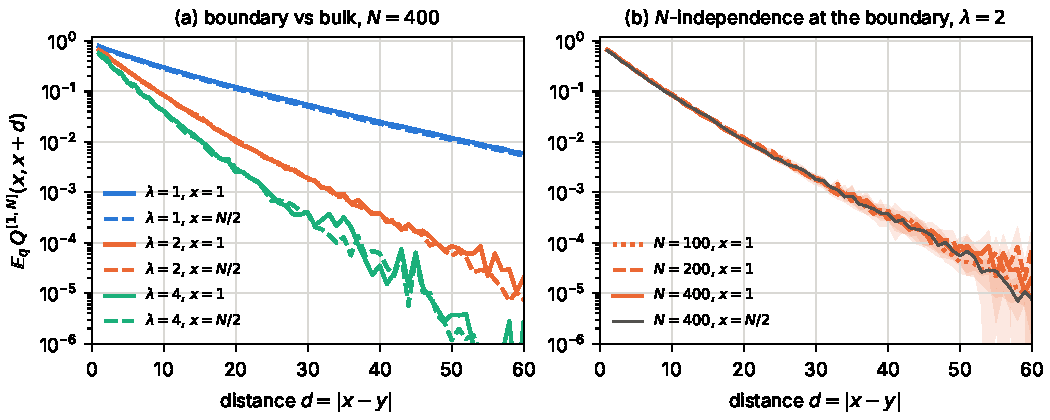
\includegraphics[width=\textwidth]{figs/correlator.pdf}
\caption{Sector-averaged eigenfunction correlator $\E_qQ^{[1,N]}_q(x,x+d)$ of
$\hq/J=-\Delta_N+\lambda\diag(q)$, over $4000$ i.i.d.\ samples of $q$ for each $(\lambda,N)$.  (a)
Boundary pairs $x=1$ (solid) and bulk pairs $x=N/2$ (dashed) at $N=400$ for $\lambda=1,2,4$.  The
boundary and bulk curves decay at the same rate, as Theorem~\ref{thm:EC} predicts.  (b) Boundary pairs
at $\lambda=2$ for $N=100,200,400$, with the bulk curve at $N=400$ (grey) and bands of $\pm2$ standard
errors: the boundary correlator does not depend on $N$.  Code:
\texttt{code/onebody\_correlator.py}; numerical values in \texttt{code/onebody\_correlator.out}.}
\label{fig:correlator}
\end{figure}

\begin{remark}[Numerical illustration]\label{rem:onebodynumerics}
\Cref{fig:correlator} shows $\E_qQ^{[1,N]}_q(x,x+d)$ for boundary and bulk pairs.  Least-squares fits of
$\log\E Q$ over $10\le d\le40$ give decay rates $\approx0.08$, $0.18$--$0.19$ and $0.21$--$0.23$ for
$\lambda=1,2,4$.  These values are the same, within the fluctuations of the fit, for boundary and bulk
pairs and for $N=100,200,400$; at $\lambda=4$ the estimates beyond $d\approx30$ are dominated by rare
samples.  The boundary values exceed the bulk values by a small but statistically significant amount at
$\lambda=1$: by $5$--$13\%$ for $1\le d\le40$ (e.g.\ $0.300$ versus $0.282$ at $d=10$, $N=400$).  The same
holds at $\lambda=2$ for $d=1$ only ($0.664$ versus $0.646$).  Otherwise the two agree within error.  For
comparison, the same code estimates $\gstar(\lambda)=\min_{E\in\Ilam}\gamma_\lambda(E)\approx0.13$, $0.34$,
$0.56$ for $\lambda=1,2,4$ (attained near $E=0$, $E\approx2.45$, $E\approx4.1$ respectively).  So the annealed
rate is well below $\gstar(\lambda)$, increasingly so as $\lambda$ grows, in line with \cref{rem:rate}(ii).
These numbers illustrate Theorem~\ref{thm:EC}; they are not used in any proof.
\end{remark}
